\documentclass[11pt,a4paper]{article}

\usepackage[utf8]{inputenc}
\usepackage[T1]{fontenc}
\usepackage[magyar]{babel}
\usepackage[a4paper,margin=2.4cm]{geometry}
\usepackage{booktabs}
\usepackage{listings}
\usepackage{xcolor}
\usepackage{enumitem}
\usepackage{tikz}
\usetikzlibrary{positioning,arrows.meta}
\usepackage{graphicx}
\usepackage[hidelinks]{hyperref}

\definecolor{codebg}{RGB}{245,245,245}

\lstset{
  basicstyle=\ttfamily\footnotesize,
  backgroundcolor=\color{codebg},
  breaklines=true,
  frame=single,
  showstringspaces=false,
  columns=fullflexible
}

\setlength{\parskip}{0.4em}
\setlength{\parindent}{0pt}

\title{\vspace{-1.5em}\textbf{Katasztrófa--Részvény Korrelációs Adatpipeline}\\[0.3em]
\large Rövid technikai dokumentáció}
\author{}
\date{}

\begin{document}
\maketitle
\vspace{-2.5em}

\section{Bevezetés}

A projekt egy teljes, end-to-end adatmérnöki pipeline, amely azt vizsgálja,
hogyan reagáltak a \textbf{biztosítótársaságok részvényárai} a
\textbf{2025. januári Los Angeles-i bozóttüzekre}. Két független adatforrást
köt össze: a NASA természeti katasztrófa eseményeit (EONET) és a biztosítók
napi tőzsdei árait. Az elemzési ablak \texttt{2024-12-01}--\texttt{2025-02-28},
amelyet egy napi ütemezett futás egészít ki friss adatokkal.

\section{A választott architektúra és indoklása}

A megoldás egy \emph{lakehouse}-jellegű mintát követ, ahol az extrakció,
transzformáció és betöltés (ETL) világosan elkülönül, így minden lépés külön
vizsgálható és újrafuttatható.

\begin{center}
\footnotesize
\textsf{NASA EONET API \; + \; yfinance/Stooq}
$\;\longrightarrow\;$ \textsf{data/raw (nyers JSON)}
$\;\longrightarrow\;$ \textsf{pandas transzformáció}
$\;\longrightarrow\;$ \textsf{data/processed (CSV)}
$\;\longrightarrow\;$ \textsf{PostgreSQL (UPSERT)}
$\;\longrightarrow\;$ \textsf{Metabase / SQL}
\end{center}
\vspace{-0.3em}
\begin{center}\footnotesize
(a teljes folyamatot az Apache Airflow DAG vezérli, \texttt{@daily} ütemezéssel)
\end{center}

\textbf{Indoklás.}
\begin{itemize}[leftmargin=1.4em,itemsep=0.1em]
  \item \textbf{Landing zone (nyers JSON):} a forrás API válaszát változatlanul
        eltároljuk, mert ez teszi lehetővé a hibakeresést és bizonyítja, hogy a
        pipeline megőrzi az eredeti, félig strukturált EONET adatot a lapítás előtt.
  \item \textbf{PostgreSQL adattárház:} robusztus, SQL-natív, könnyen
        konténerizálható, és az \texttt{ON CONFLICT} (UPSERT) szemantikával az
        idempotens betöltés alapja.
  \item \textbf{Apache Airflow:} explicit, DAG-alapú orkesztráció
        újrapróbálkozással, ütemezéssel és megfigyelhetőséggel; a lépések külön
        task-okra bonthatók, a transzformáció és betöltés dinamikus task
        mappinggel (\texttt{.expand()}) párhuzamosítható.
  \item \textbf{Adatforrások:} az EONET ingyenes és mélyen beágyazott JSON-t ad
        (félig strukturált forrás); a részvényárakat elsődlegesen az
        \texttt{yfinance} adja, amely Stooq $\rightarrow$ Alpha Vantage
        $\rightarrow$ seed CSV $\rightarrow$ szimuláció fallback-láncra épül, így
        a futás külső kiesés esetén sem szakad meg.
  \item \textbf{Docker Compose:} egyetlen paranccsal reprodukálja a teljes
        környezetet (PostgreSQL, Airflow, Metabase); minden paraméter a
        \texttt{.env} fájlban van (nincs hardcode-olt érték).
\end{itemize}

\textbf{Idempotencia és ütemezés.} A betöltés UPSERT-tel történik, a
transzformáció fájlrendszer-szintű gyorsítótárat használ, így ugyanazon nap
újrafuttatása nem hoz létre duplikátumot. A DAG adaptív: ütemezett futáskor
csak az előző napot dolgozza fel (gyors marad), kézi
\texttt{\{"backfill": true\}} konfigurációval pedig a teljes történeti ablakot.

\section{Adatmodell (csillagséma)}

Az adattárház Kimball-stílusú dimenziós modellt használ \textbf{két ténytáblával},
amelyek közös (konformált) dimenziókon osztoznak. A kettős ténytáblás kialakítás
külön kezeli a két szemcsézettséget: a részvényár csak kereskedési napokon
létezik, a katasztrófa-közelség viszont minden naptári napon, városonként.

\begin{figure}[ht]
\centering
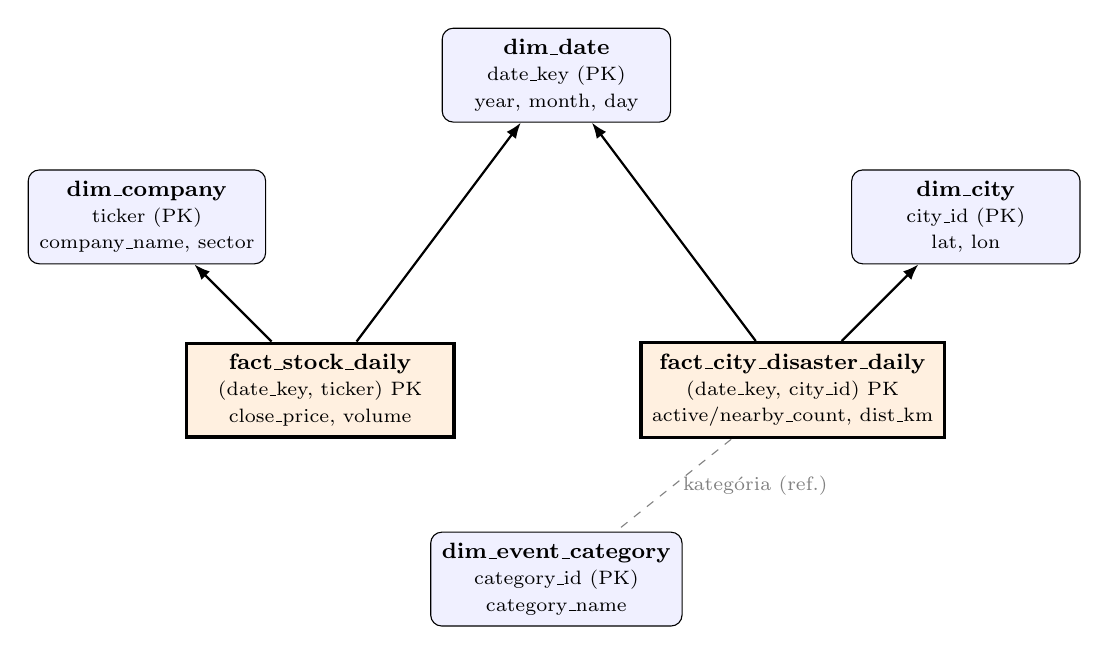
\begin{tikzpicture}[
  font=\footnotesize,
  dim/.style={rectangle, draw, rounded corners, fill=blue!6, align=center, inner sep=4pt, minimum width=2.9cm},
  fact/.style={rectangle, draw, very thick, fill=orange!12, align=center, inner sep=4pt, minimum width=3.4cm},
  link/.style={-{Latex[length=2mm]}, thick},
  ref/.style={dashed, gray}
]
% dimensions
\node[dim] (company) at (-5.2,1.6) {\textbf{dim\_company}\\\scriptsize ticker (PK)\\\scriptsize company\_name, sector};
\node[dim] (date)    at (0,3.4)    {\textbf{dim\_date}\\\scriptsize date\_key (PK)\\\scriptsize year, month, day};
\node[dim] (city)    at (5.2,1.6)  {\textbf{dim\_city}\\\scriptsize city\_id (PK)\\\scriptsize lat, lon};
\node[dim] (cat)     at (0,-3.0)   {\textbf{dim\_event\_category}\\\scriptsize category\_id (PK)\\\scriptsize category\_name};
% facts
\node[fact] (stock)  at (-3.0,-0.6) {\textbf{fact\_stock\_daily}\\\scriptsize (date\_key, ticker) PK\\\scriptsize close\_price, volume};
\node[fact] (disas)  at (3.0,-0.6)  {\textbf{fact\_city\_disaster\_daily}\\\scriptsize (date\_key, city\_id) PK\\\scriptsize active/nearby\_count, dist\_km};
% links
\draw[link] (stock) -- (company);
\draw[link] (stock) -- (date);
\draw[link] (disas) -- (date);
\draw[link] (disas) -- (city);
\draw[ref]  (disas) -- (cat) node[midway,right,gray]{\scriptsize kategória (ref.)};
\end{tikzpicture}
\caption{Csillagséma: 2 ténytábla (narancs) + 4 konformált dimenzió (kék).}
\end{figure}

A \texttt{dim\_company} a betöltés során automatikusan feltöltődik a
ténytáblában szereplő tickerekből, így egy friss adattárház is teljesíti a
\texttt{fact\_stock\_daily} idegenkulcs-megszorítását. A két ténytáblát
elemzéshez SQL nézetek kötik össze (pl. \texttt{vw\_stock\_disaster\_price\_movement},
amely \texttt{LAG()} ablakfüggvénnyel napi \% árváltozást is számol).

\section{A pipeline futásának eredménye}

A \texttt{backfill} futás sikeresen lefutott (1083 task-példány, mind
\emph{success}), és valós adatot töltött be: \textbf{396 részvénysort}
(6 biztosító × 60 kereskedési nap) és \textbf{910 katasztrófasort} a
\texttt{2024-12-01}--\texttt{2025-02-28} ablakban. Az alábbi lekérdezés az
Allstate (ALL) reakcióját mutatja a tűzvész körül:

\begin{lstlisting}[language=SQL]
SELECT date_key, stock_close_price, pct_close_change,
       nearby_disaster_count, nearest_disaster_distance_km
FROM vw_stock_disaster_price_movement
WHERE ticker = 'ALL' AND city_id = 'US-LOS_ANGELES'
  AND date_key BETWEEN '2025-01-03' AND '2025-01-15'
ORDER BY date_key;
\end{lstlisting}

\begin{table}[ht]
\centering\footnotesize
\begin{tabular}{@{}lrrrr@{}}
\toprule
\textbf{date\_key} & \textbf{close (USD)} & \textbf{pct \%} & \textbf{nearby} & \textbf{dist\_km} \\
\midrule
2025-01-03 & 191.45 & -0.26 & 0 & 11905.52 \\
2025-01-06 & 185.91 & \textbf{-2.89} & 1 & 26.48 \\
2025-01-07 & 186.04 & 0.07 & 1 & 20.06 \\
2025-01-08 & 191.80 & 3.10 & 1 & 36.49 \\
2025-01-10 & 180.99 & \textbf{-5.64} & 0 & 3580.18 \\
2025-01-13 & 182.54 & 0.86 & 0 & 12281.47 \\
2025-01-14 & 186.81 & 2.34 & 0 & 5960.71 \\
2025-01-15 & 188.03 & 0.65 & 0 & 3574.70 \\
\bottomrule
\end{tabular}
\caption{Allstate (ALL) napi záróár és \%-os változás a tűzvész idején.}
\end{table}

\textbf{Értelmezés.} A bozóttüzek 2025. január 6--8. között Los Angelestől
mindössze \mbox{20--36 km}-re voltak aktívak (\texttt{nearby\_disaster\_count} = 1).
Ezzel egyidőben az Allstate árfolyama január 6-án $-2{,}89\%$-ot, majd január
10-én $-5{,}64\%$-ot esett (191,80 USD $\rightarrow$ 180,99 USD), a forgalom
pedig $\sim$2,4 millióról $\sim$4,6 millió darabra ugrott -- ez egyértelmű
piaci reakció a várható kárkifizetésekre. Havi bontásban a januári átlagos
aktív katasztrófaszám volt a legmagasabb az időszakban:

\begin{table}[ht]
\centering\footnotesize
\begin{tabular}{@{}rrrrr@{}}
\toprule
\textbf{év} & \textbf{hónap} & \textbf{átl. aktív kat.} & \textbf{átl. LA-közeli} & \textbf{átl. záróár} \\
\midrule
2024 & 12 & 7.7  & 0.05 & 250.45 \\
2025 & 1  & \textbf{11.1} & 0.20 & 245.95 \\
2025 & 2  & 10.3 & 0.00 & 254.72 \\
\bottomrule
\end{tabular}
\caption{Havi katasztrófa-kitettség és átlagos biztosítói záróár.}
\end{table}

\textbf{Napi ütemezett futások.} A történeti \texttt{backfill} mellett a DAG
\texttt{@daily} ütemezéssel önállóan is fut: minden ütemezett futás az
előző napot tölti be (adaptív ablak), így az adattárház naprakész marad.
A \ref{fig:airflow-daily}.~ábra a két legutóbbi napi futást mutatja az
Airflow gráfnézetében -- mindkét futás \emph{minden} taskja sikeresen
lefutott (\texttt{check\_api} $\rightarrow$
\texttt{extract\_stocks}/\texttt{extract\_eonet} $\rightarrow$
\texttt{transform} $\rightarrow$ \texttt{load}), a dinamikus task mapping
(\texttt{[6]}) pedig a hat biztosító párhuzamos feldolgozását jelzi.

\begin{figure}[ht]
\centering
\begin{minipage}[t]{0.49\textwidth}
  \centering
  \fbox{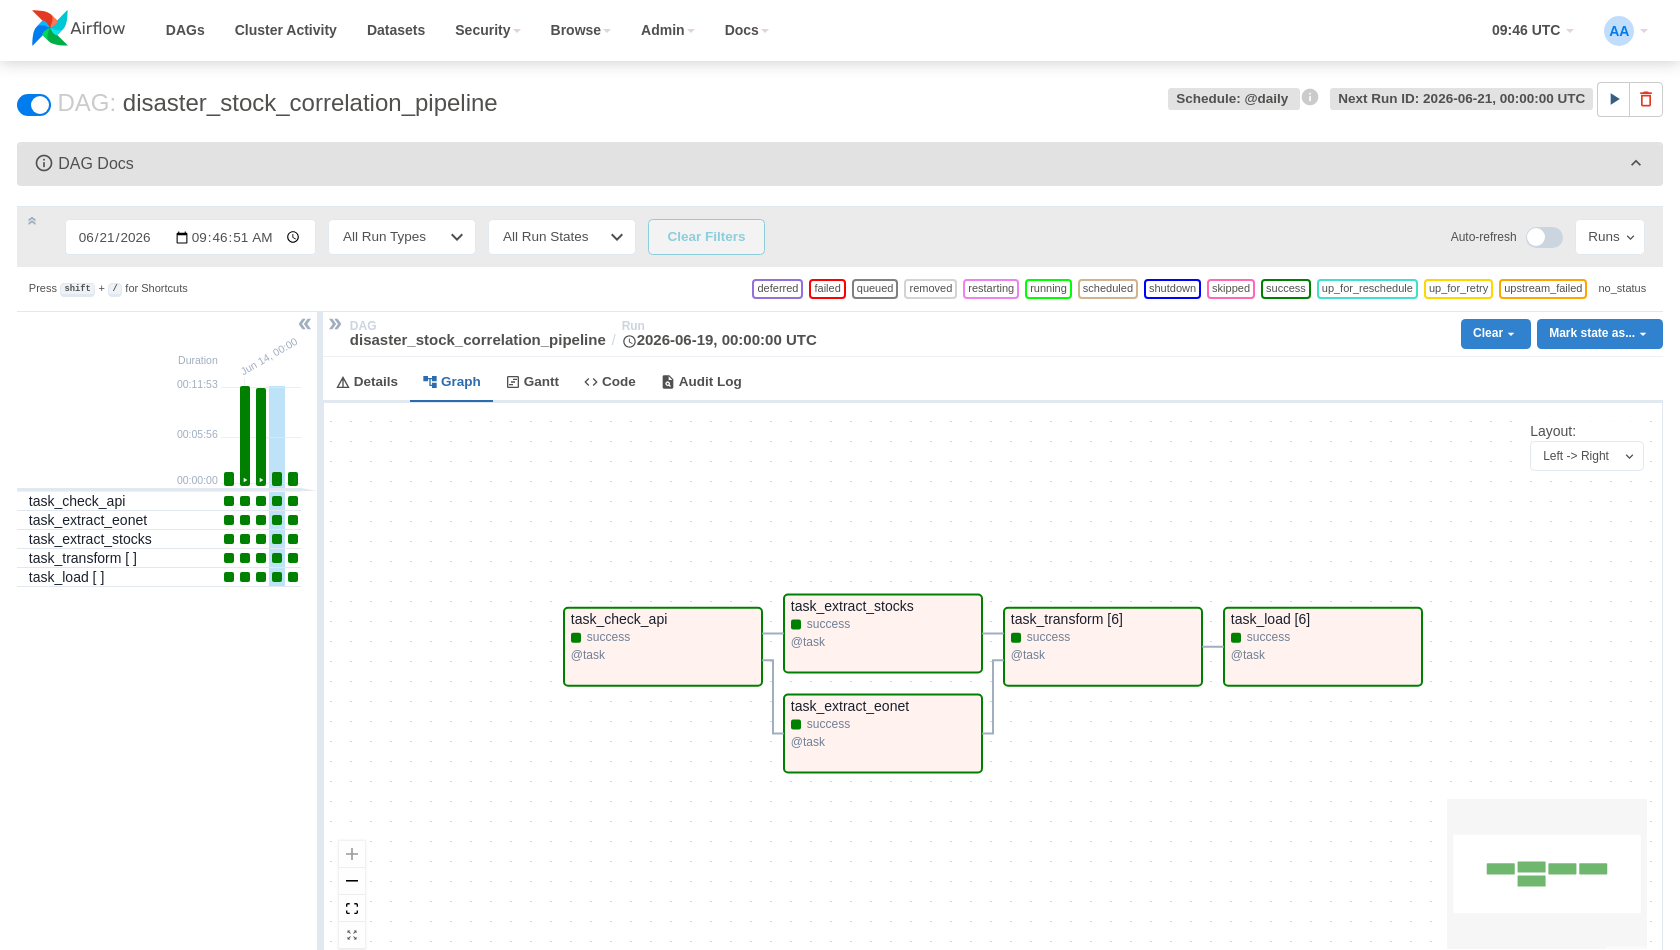
\includegraphics[width=\linewidth]{docs/img/airflow_run_2026-06-19.png}}\\[2pt]
  {\scriptsize (a) \texttt{scheduled\_\_2026-06-19} futás}
\end{minipage}\hfill
\begin{minipage}[t]{0.49\textwidth}
  \centering
  \fbox{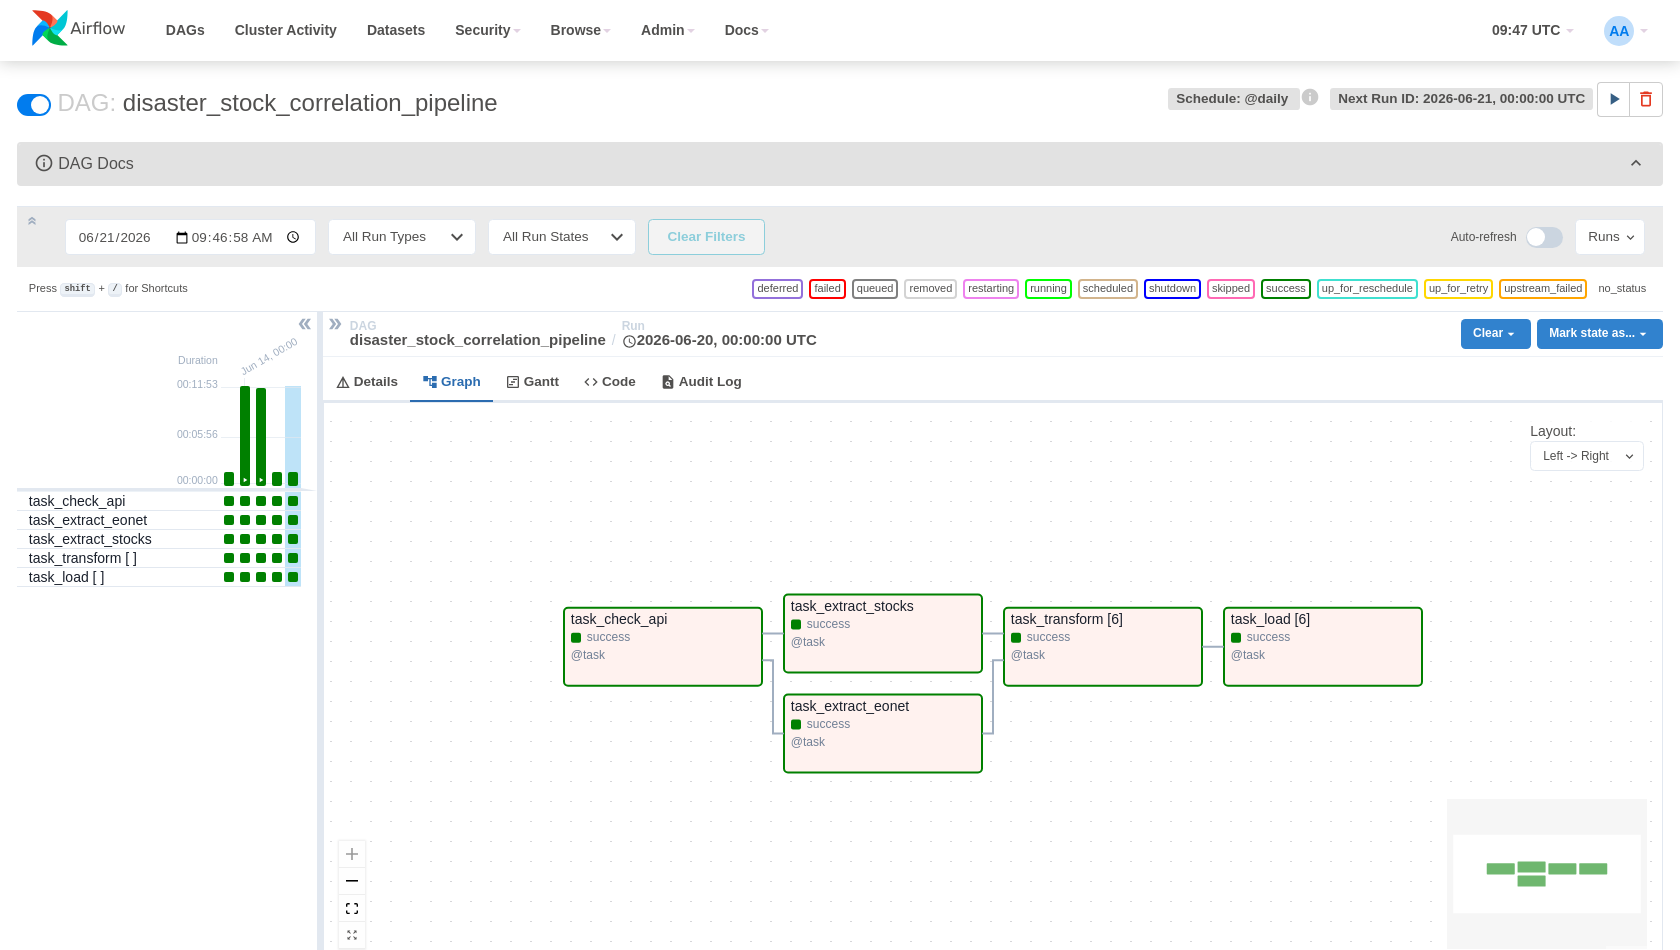
\includegraphics[width=\linewidth]{docs/img/airflow_run_2026-06-20.png}}\\[2pt]
  {\scriptsize (b) \texttt{scheduled\_\_2026-06-20} futás}
\end{minipage}
\caption{A két napi ütemezett (\texttt{@daily}) Airflow-futás gráfnézete --
minden task állapota \emph{success}.}
\label{fig:airflow-daily}
\end{figure}

Az eredmények a Metabase \emph{LA Wildfire Insurance Impact} dashboardon
vizualizálva is elérhetők (a Metabase nyitóoldalára kitűzve, lásd
\ref{fig:dashboard}. ábra): biztosítói záróár-idősorok, az LA-közeli
katasztrófák száma (jól látható a januári kiugrás), napi \%-os árváltozás,
városonkénti kitettség, a csúcs-katasztrófaszám és egy részletező táblázat.

\begin{figure}[ht]
\centering
\fbox{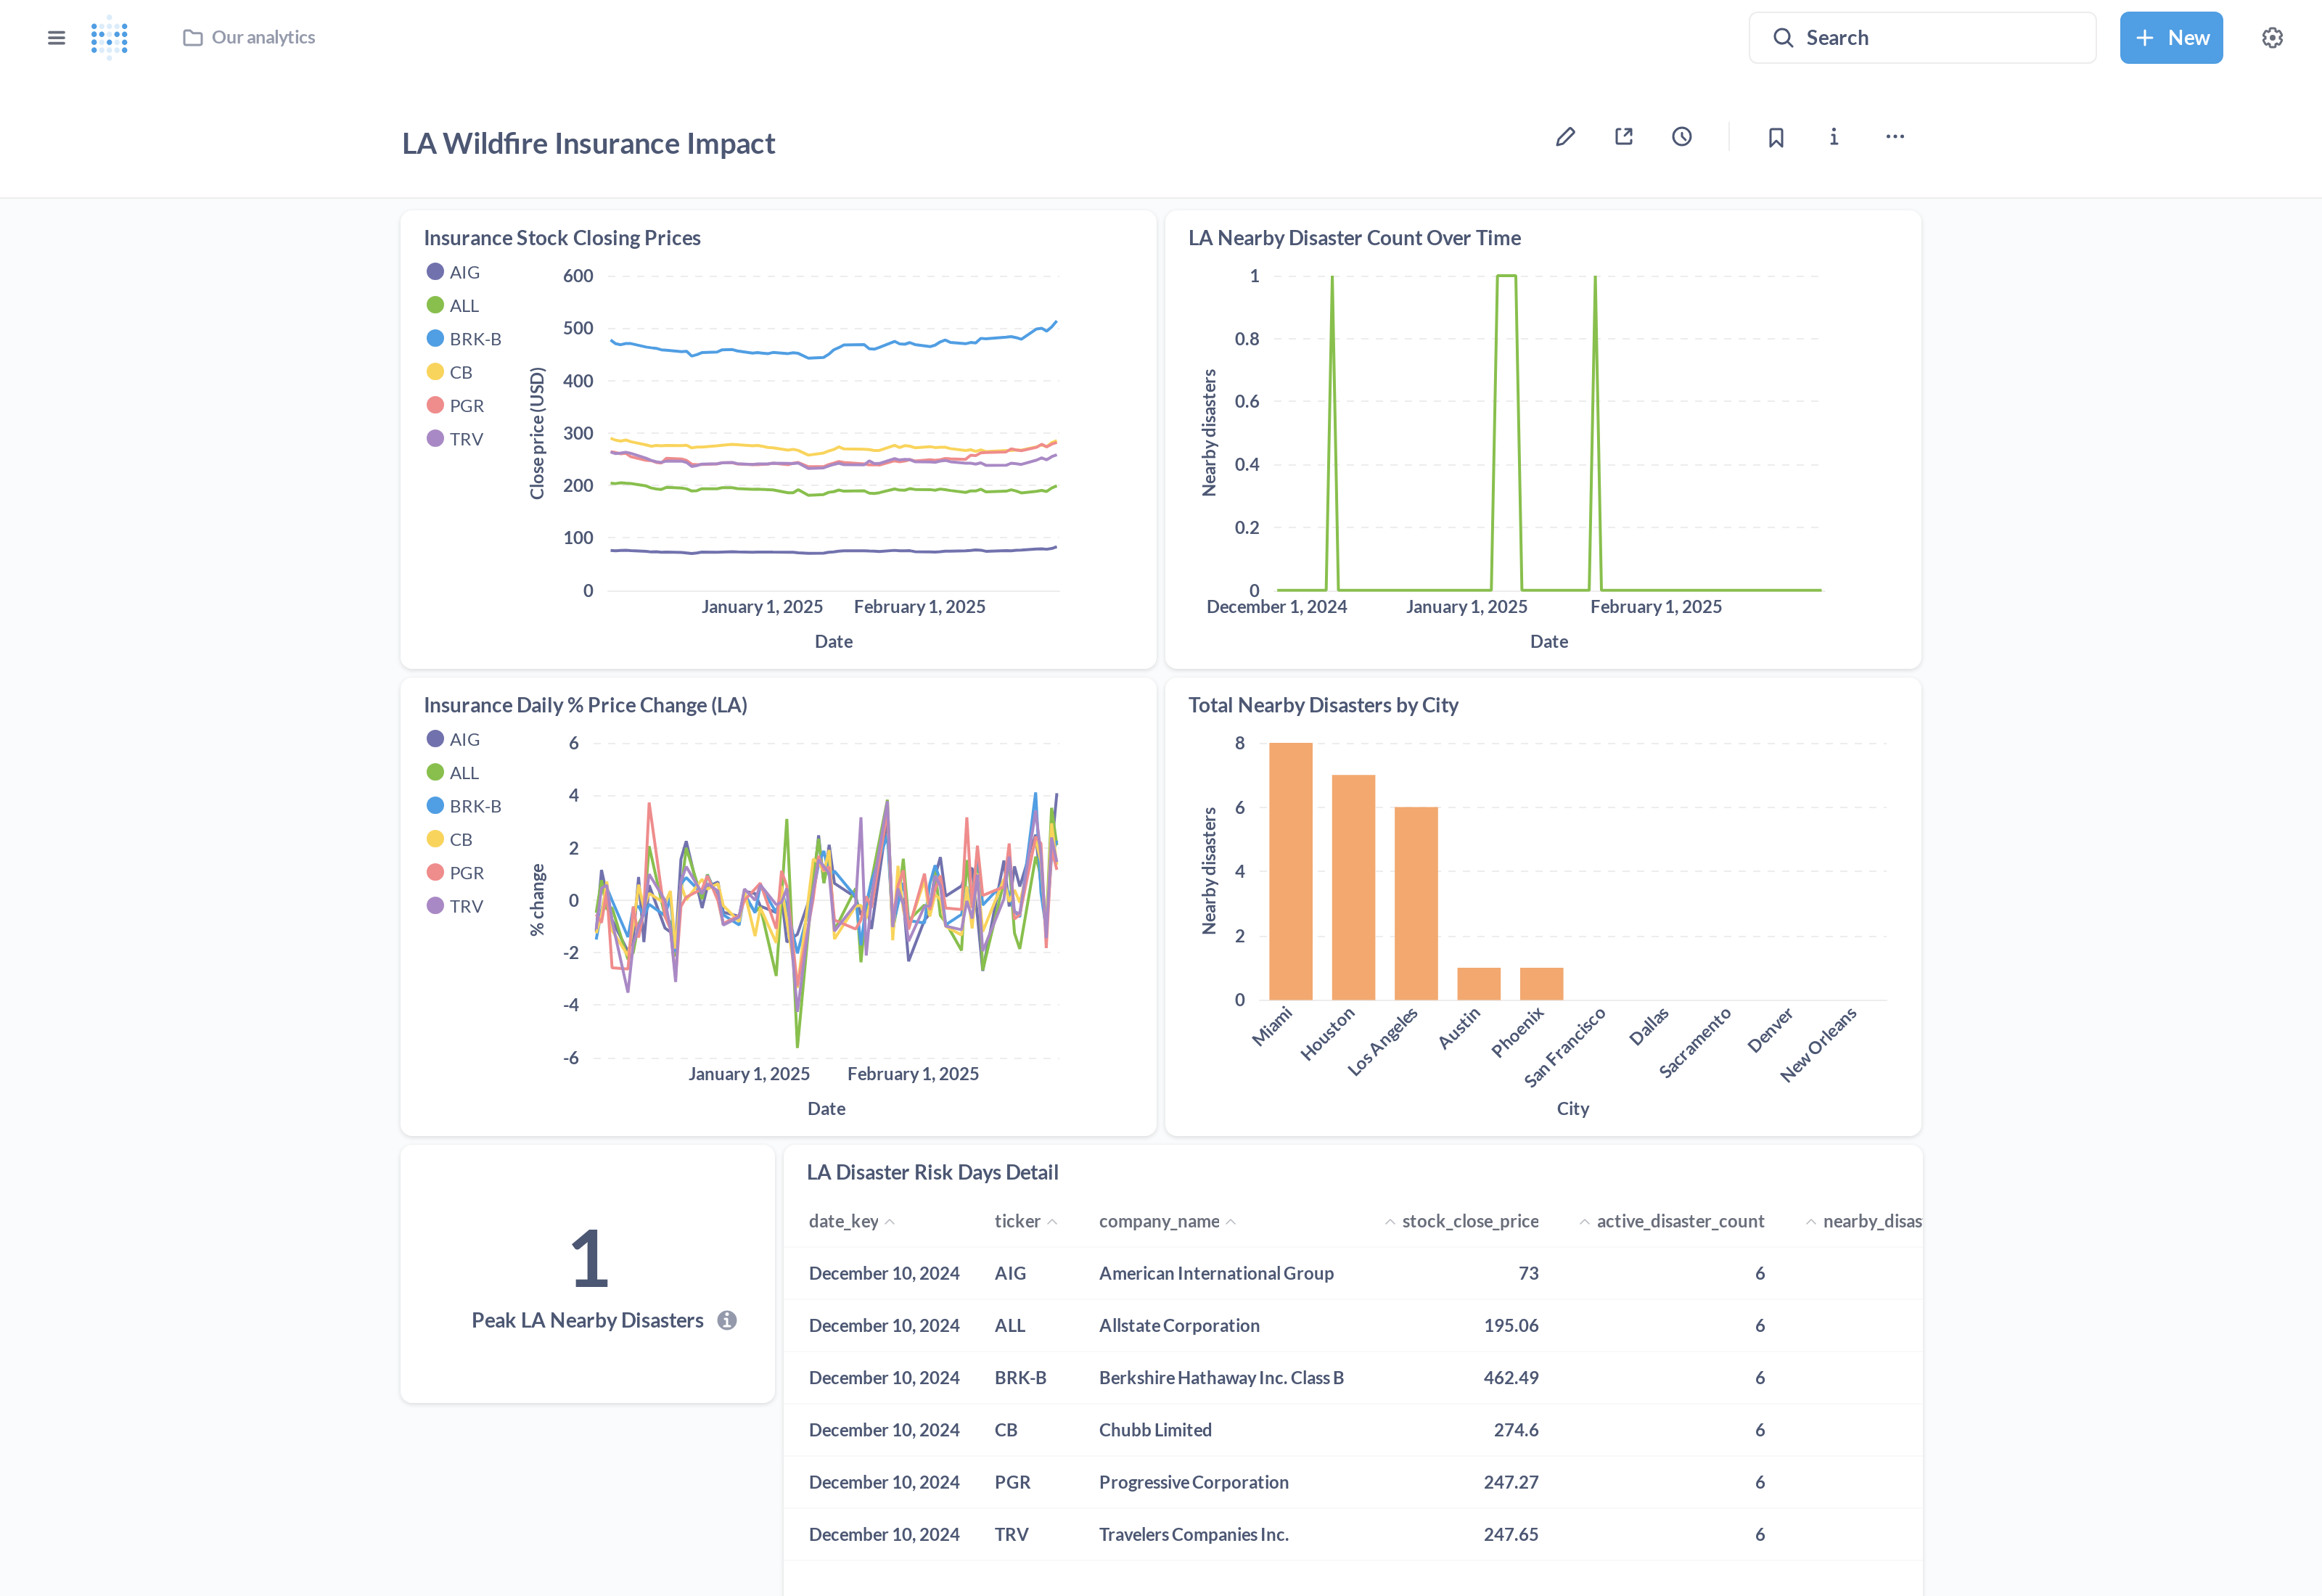
\includegraphics[width=0.98\textwidth]{docs/img/dashboard.png}}
\caption{A Metabase \emph{LA Wildfire Insurance Impact} dashboard a valós,
betöltött adatokkal.}
\label{fig:dashboard}
\end{figure}

A további dokumentált SQL lekérdezések az \texttt{ANALYTICAL\_QUERIES.md}
fájlban találhatók, a futtatás lépései pedig a \texttt{README.md}-ben.

\end{document}
